\section*{Results}

\subsection*{First part}

\begin{center}
    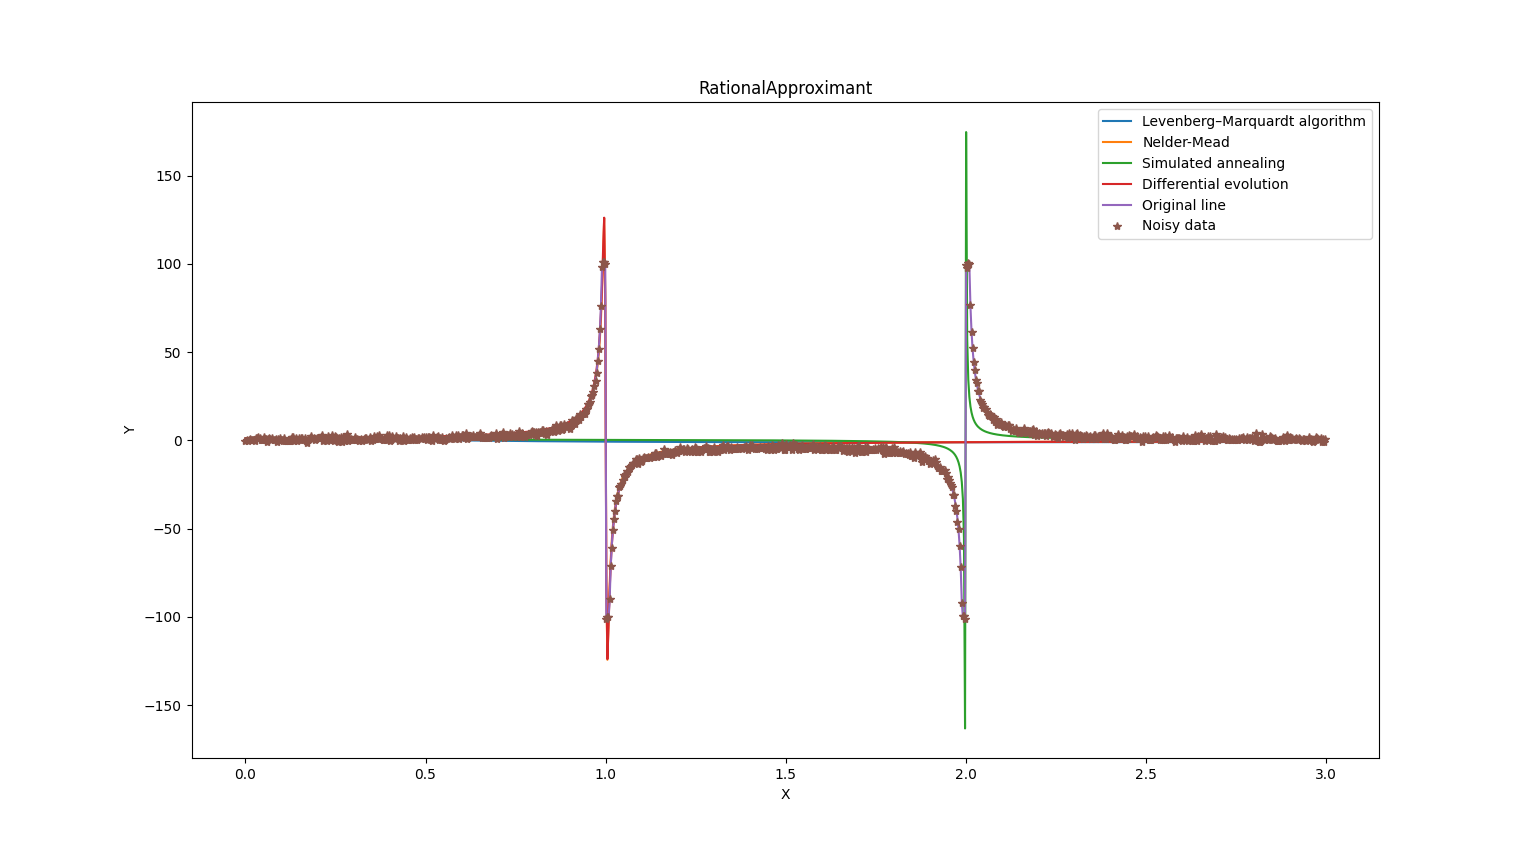
\includegraphics[width=0.85\textwidth]{../results/rational_1_1_1_1.png}
    \captionof{figure}{Approximation with $(1, 1, 1, 1)$ initial guess}
    \label{fig:aprox_first}
\end{center}

\begin{center}
    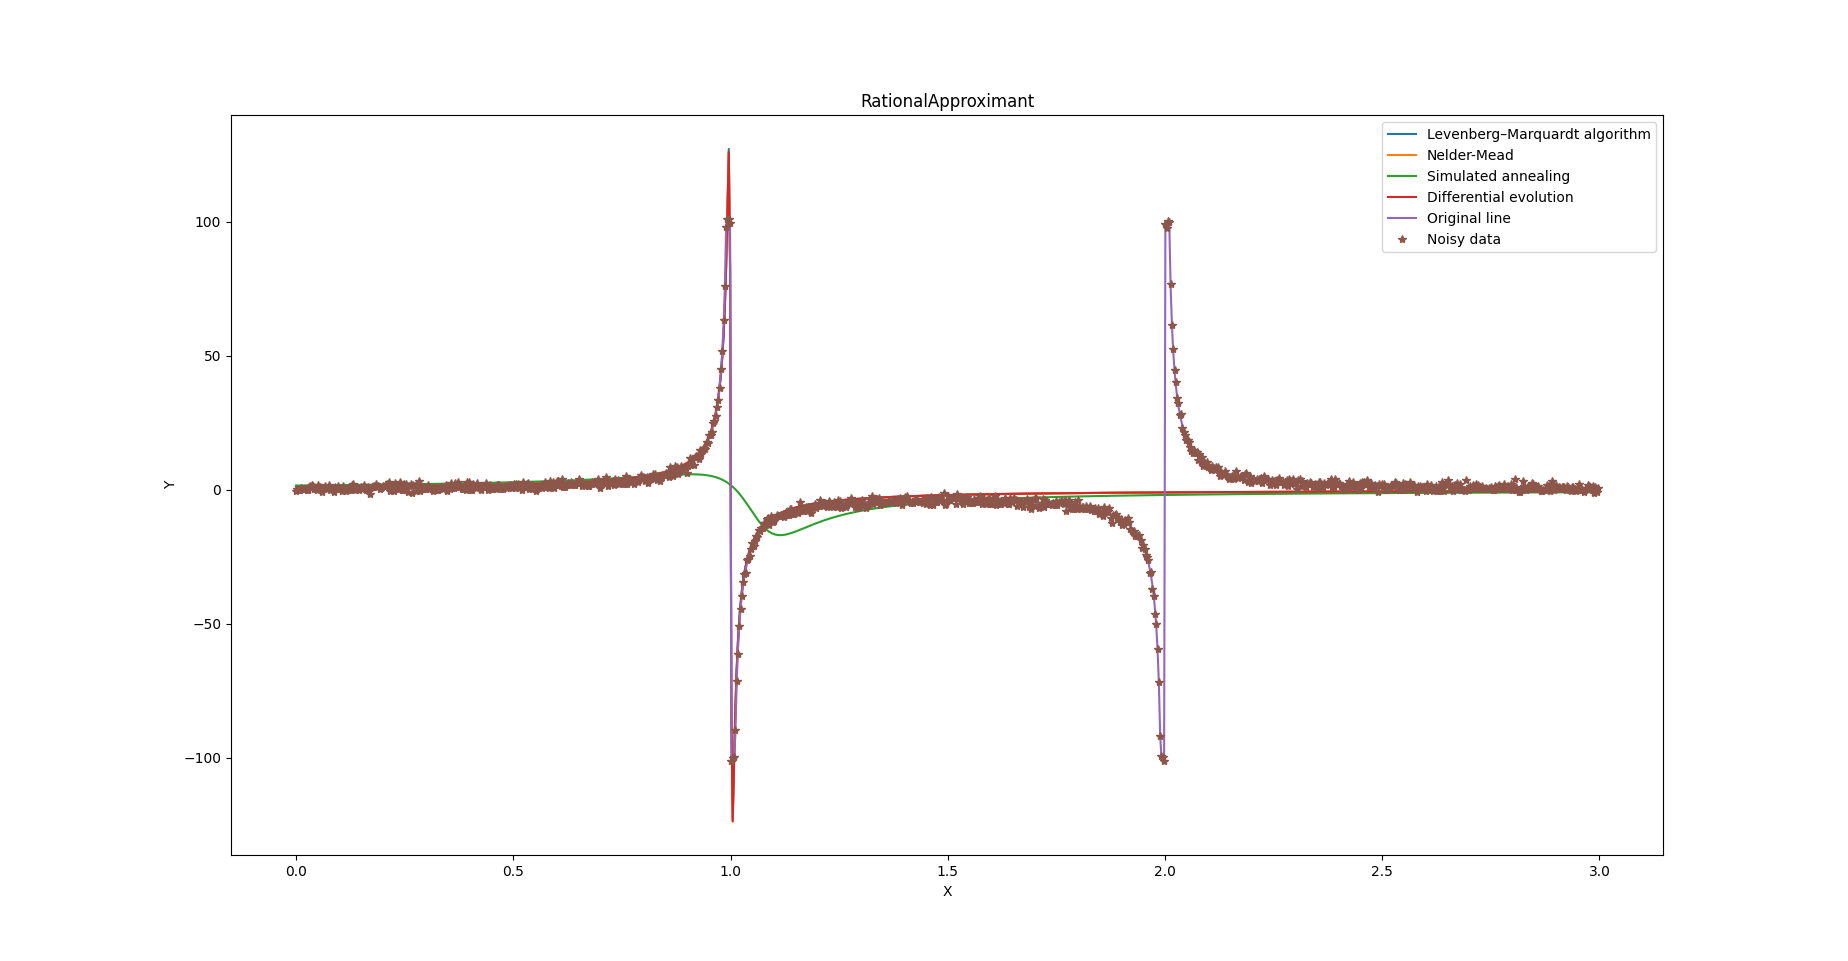
\includegraphics[width=0.85\textwidth]{../results/rational_second.png}
    \captionof{figure}{Approximation with $(-1, 1, -2, 1)$ initial guess}
    \label{fig:aprox_second}
\end{center}

In Figure \ref{fig:aprox_first} and Table \ref{tab:aprox_first} results of approximation with initial guess $(1, 1, 1, 1)$ for approximant parameters are presented. 
The Nelder-Mead and Differential evolution converged to similar sollution that approximated the first function break. The Simulated anneling algorithm was able to converge to
another suboptimal sollution that approximate the second function break. Levenberg-Marquadt did not converge to sollution with adequate squared error and in fugure is presented by linear-like function.

In terms of squared error the best results are shown by Nelder-Mead (NM) and Differential evolution (DE) algorithms, although Nelder-Mead got slightly better sollution.
As well as that it required the least number of function evaluations for convergence in that case. DE required the least number of iterations (6), although it caused by size of population
used in algorithm and higher number function evalutions. That is why NM can be considered the most effective in that case in terms of calculations. 

\begin{table*}[h!]
    \begin{center}
        \caption{Optimization results for (1, 1, 1, 1) ininital guess}
        \label{table:direct-methods}
        \begin{tabular}{|c|c|c|c|c|}
            \label{tab:aprox_first}
            \textbf{Algorithm} & \textbf{$a, b, c, d$} & \textbf{$(\hat{y} - y)^2$} & \textbf{Evaluations} & \textbf{Iterations}\\
            \hline
            Real & (0, 1, -3, 2) & 966.36 & &\\
            Levenberg-Marquardt & (-3.2, 1.8, -0.5, 1.4) & 266530 & 28 & 28 \\
            Nelder-Mead & (-0.9, 0.9, -2.0, 1.0) & \textbf{136234} & \textbf{801} & 479 \\
            Simulated annealing & (1.5, -2.2, -0.6, -2.7) & 197900 & 8001 & 1000 \\
            Differential evolution &  (-1.0, 1.0, -2.0, 1.0) & 136468 & 1045 & \textbf{6} \\
        \end{tabular}
    \end{center}
\end{table*}

\begin{table*}[h!]
    \begin{center}
        \caption{Optimization results for first- and second-order methods}
        \label{tab:aprox_second}
        \begin{tabular}{|c|c|c|c|c|}
            \textbf{Algorithm} & \textbf{$a, b$} & \textbf{$(\hat{y} - y)^2$} & \textbf{Evaluations} & \textbf{Iterations}\\
            \hline
            Real & (0, 1, -3, 2) & 966.36 & &\\
            Levenberg-Marquardt & (-0.9, 0.9, -2.0, 1.0) & 136240 & \textbf{26} & 26 \\
            Nelder-Mead & (-1.0, 1.0, -2.0, 1.0) & 136265 & 325 & 187 \\
            Simulated annealing & (-1.7, 1.7, -2.1, 1.13) & 250943 & 8001 & 1000 \\
            Differential evolution &  (-0.9, 0.9, -2.0, 1.0) & \textbf{136232} & 1010 & \textbf{6} \\
        \end{tabular}
    \end{center}
\end{table*}

In Figure \ref{fig:aprox_second} and Table \ref{tab:aprox_second} results of approximation with initial guess $(-11, 1, -2, 1)$ for approximant parameters are presented. 
That initial guess was choosed as approximation close to the sollution from previous experiment. The most significant thing to be mentioned in thing in that case is
that LMA was able to converge to sollution that approximates sollution with first function brake with error lower than NM-algorithm with much lower number of function evalutions.
Another thing to be mentioned is that in case of that initial guess Simulated anneling was unable to converge to previous sollution as well as to sollution with first function break, although
it did not converge to linear-like funciton on interval and has some observable unlinearity in neighbourhood of first line break.

\subsection*{Second part}

In this part \href{https://people.sc.fsu.edu/~jburkardt/datasets/cities/wg22_dist.txt}{WG22} dataset was used that contains distances between 22 cities in Western Germany.

In figures \ref{fig:tsp_0}, \ref{fig:tsp_1} the first and last (50000th) iteration of simulated anneling for TSP optimization are shown.
As it can be seen from figures the overall route cost in suboptimal sollution is in about 3 times lower. The simulated annealing allows to receive suboptimal
sollution wich much less computations (50000 iterations) then brute force that has $O(n - 1)$ complexity. In case of WG22 it is $21! \approx 5 * 10^{19}$.

\begin{center}
    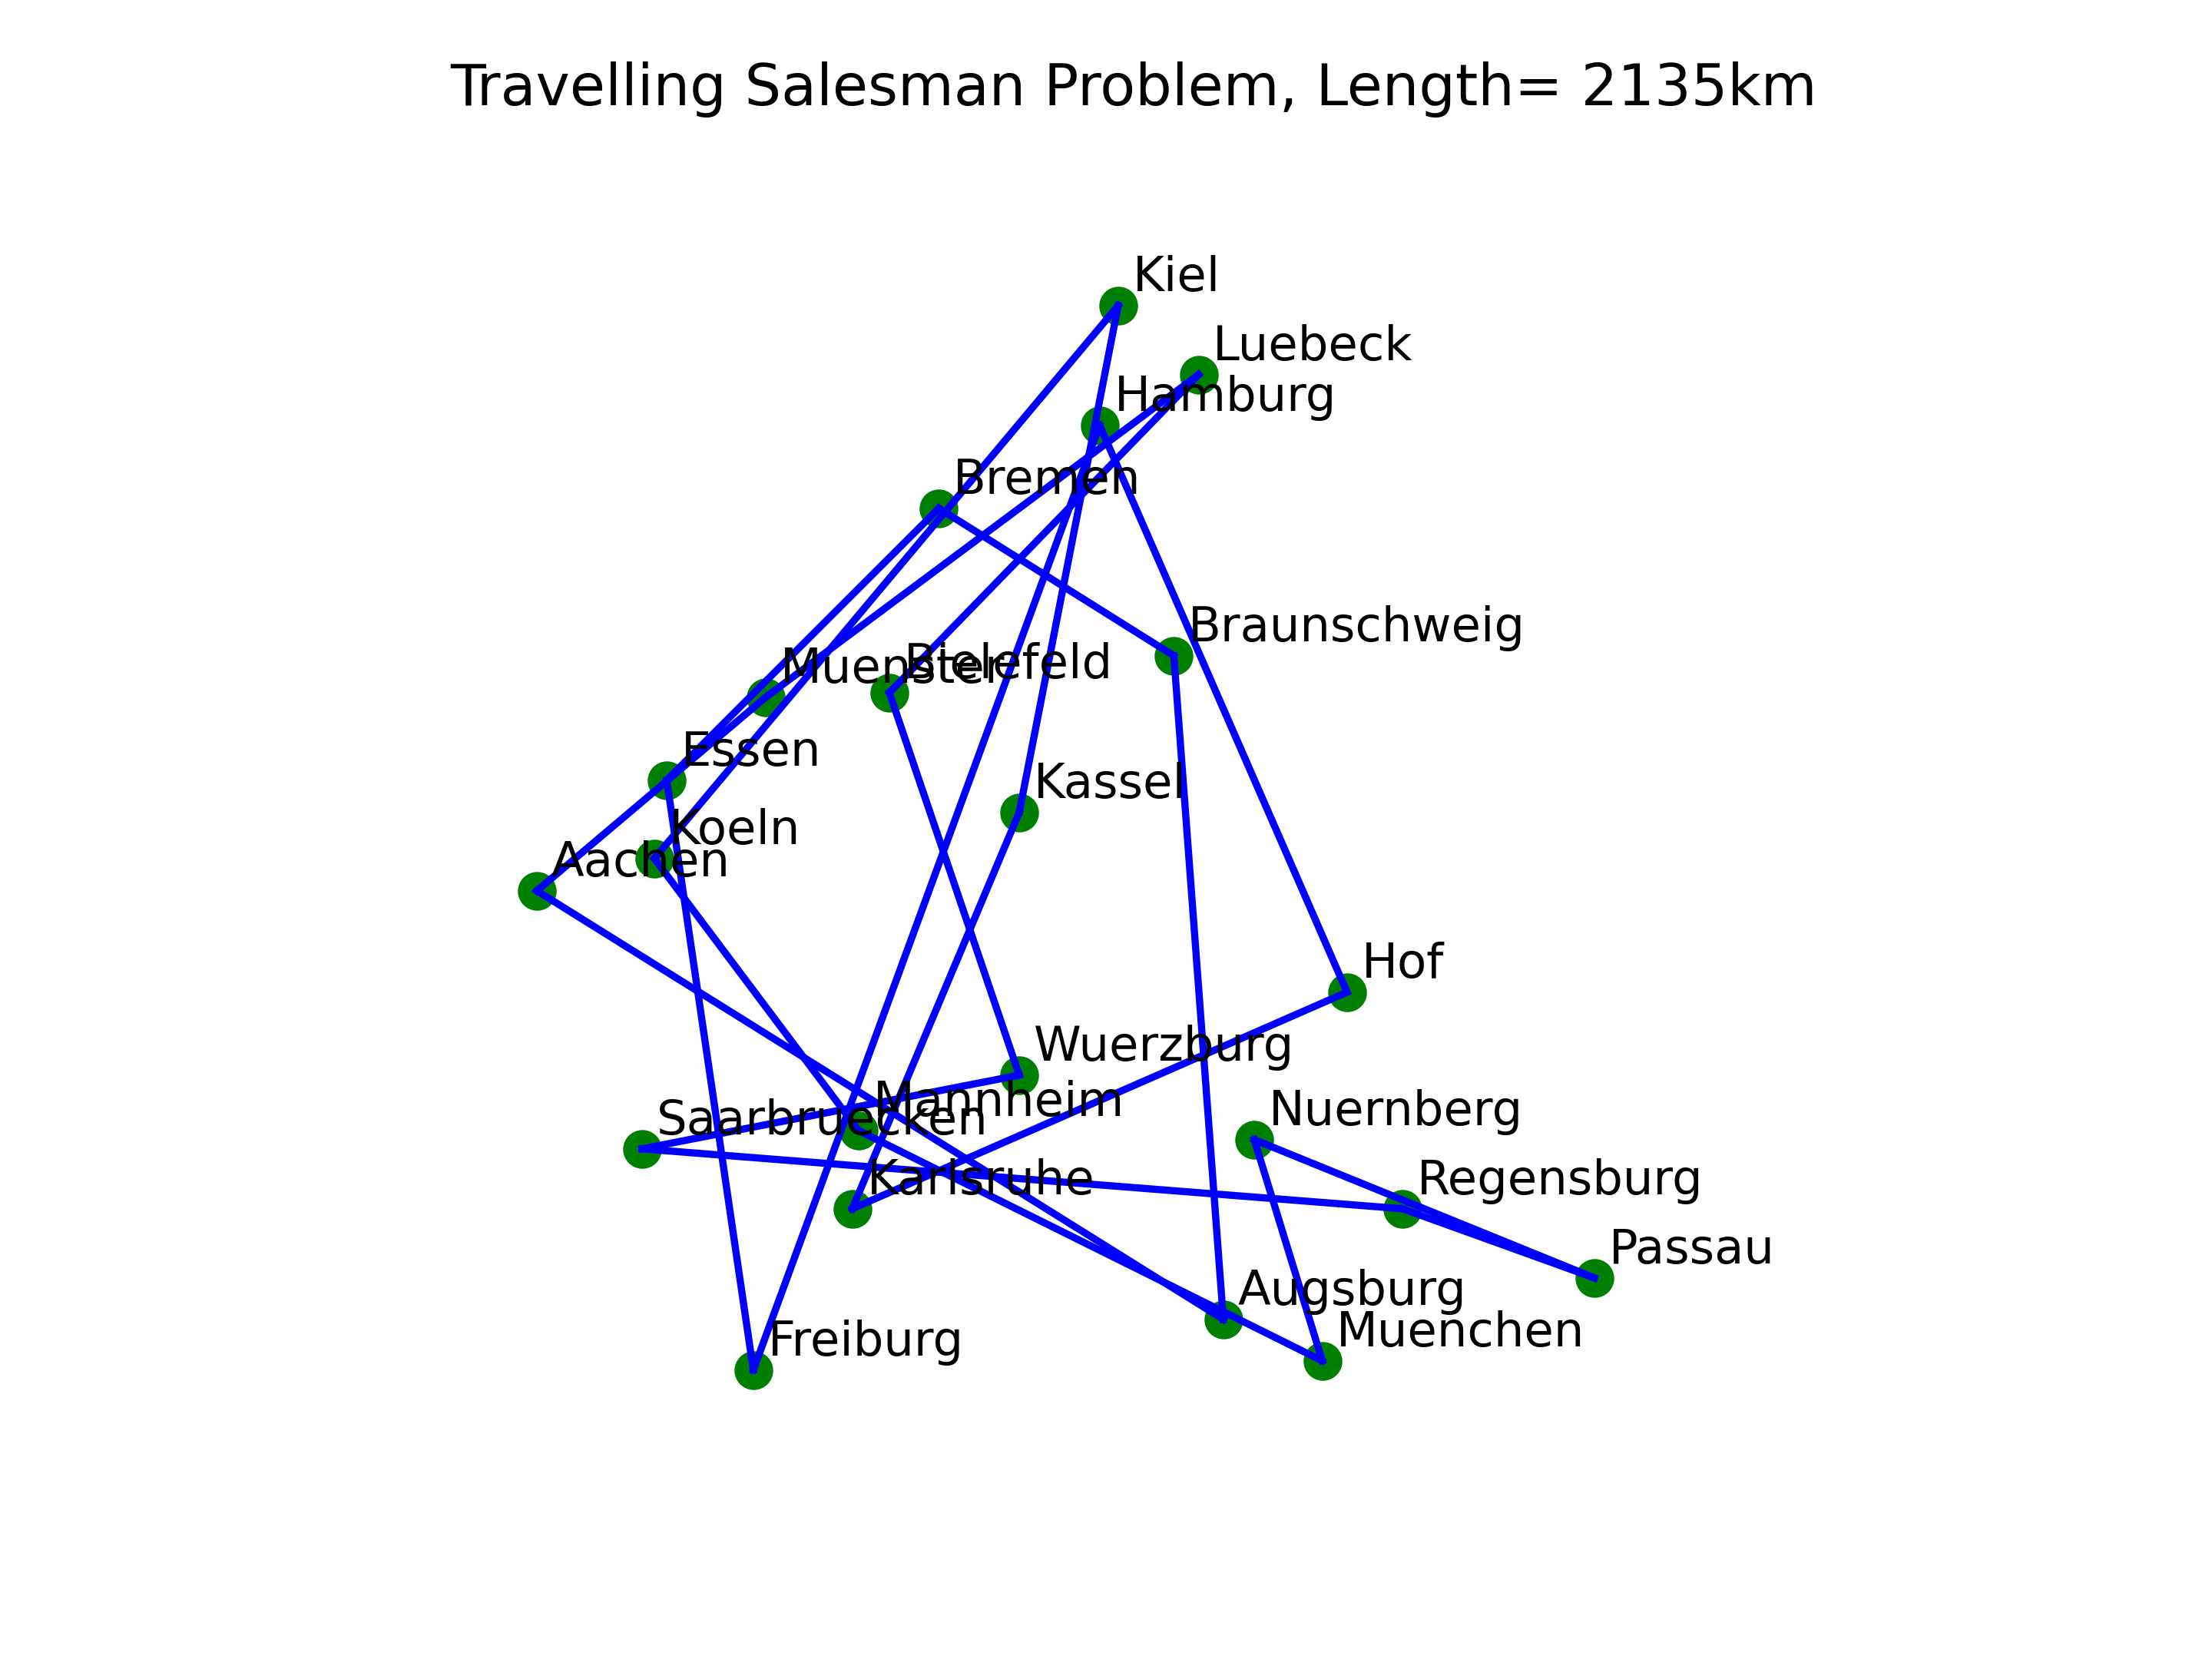
\includegraphics[width=0.80\textwidth]{../results/tsp_0.png}
    \captionof{figure}{Initial route}
    \label{fig:tsp_0}
\end{center}

\begin{center}
    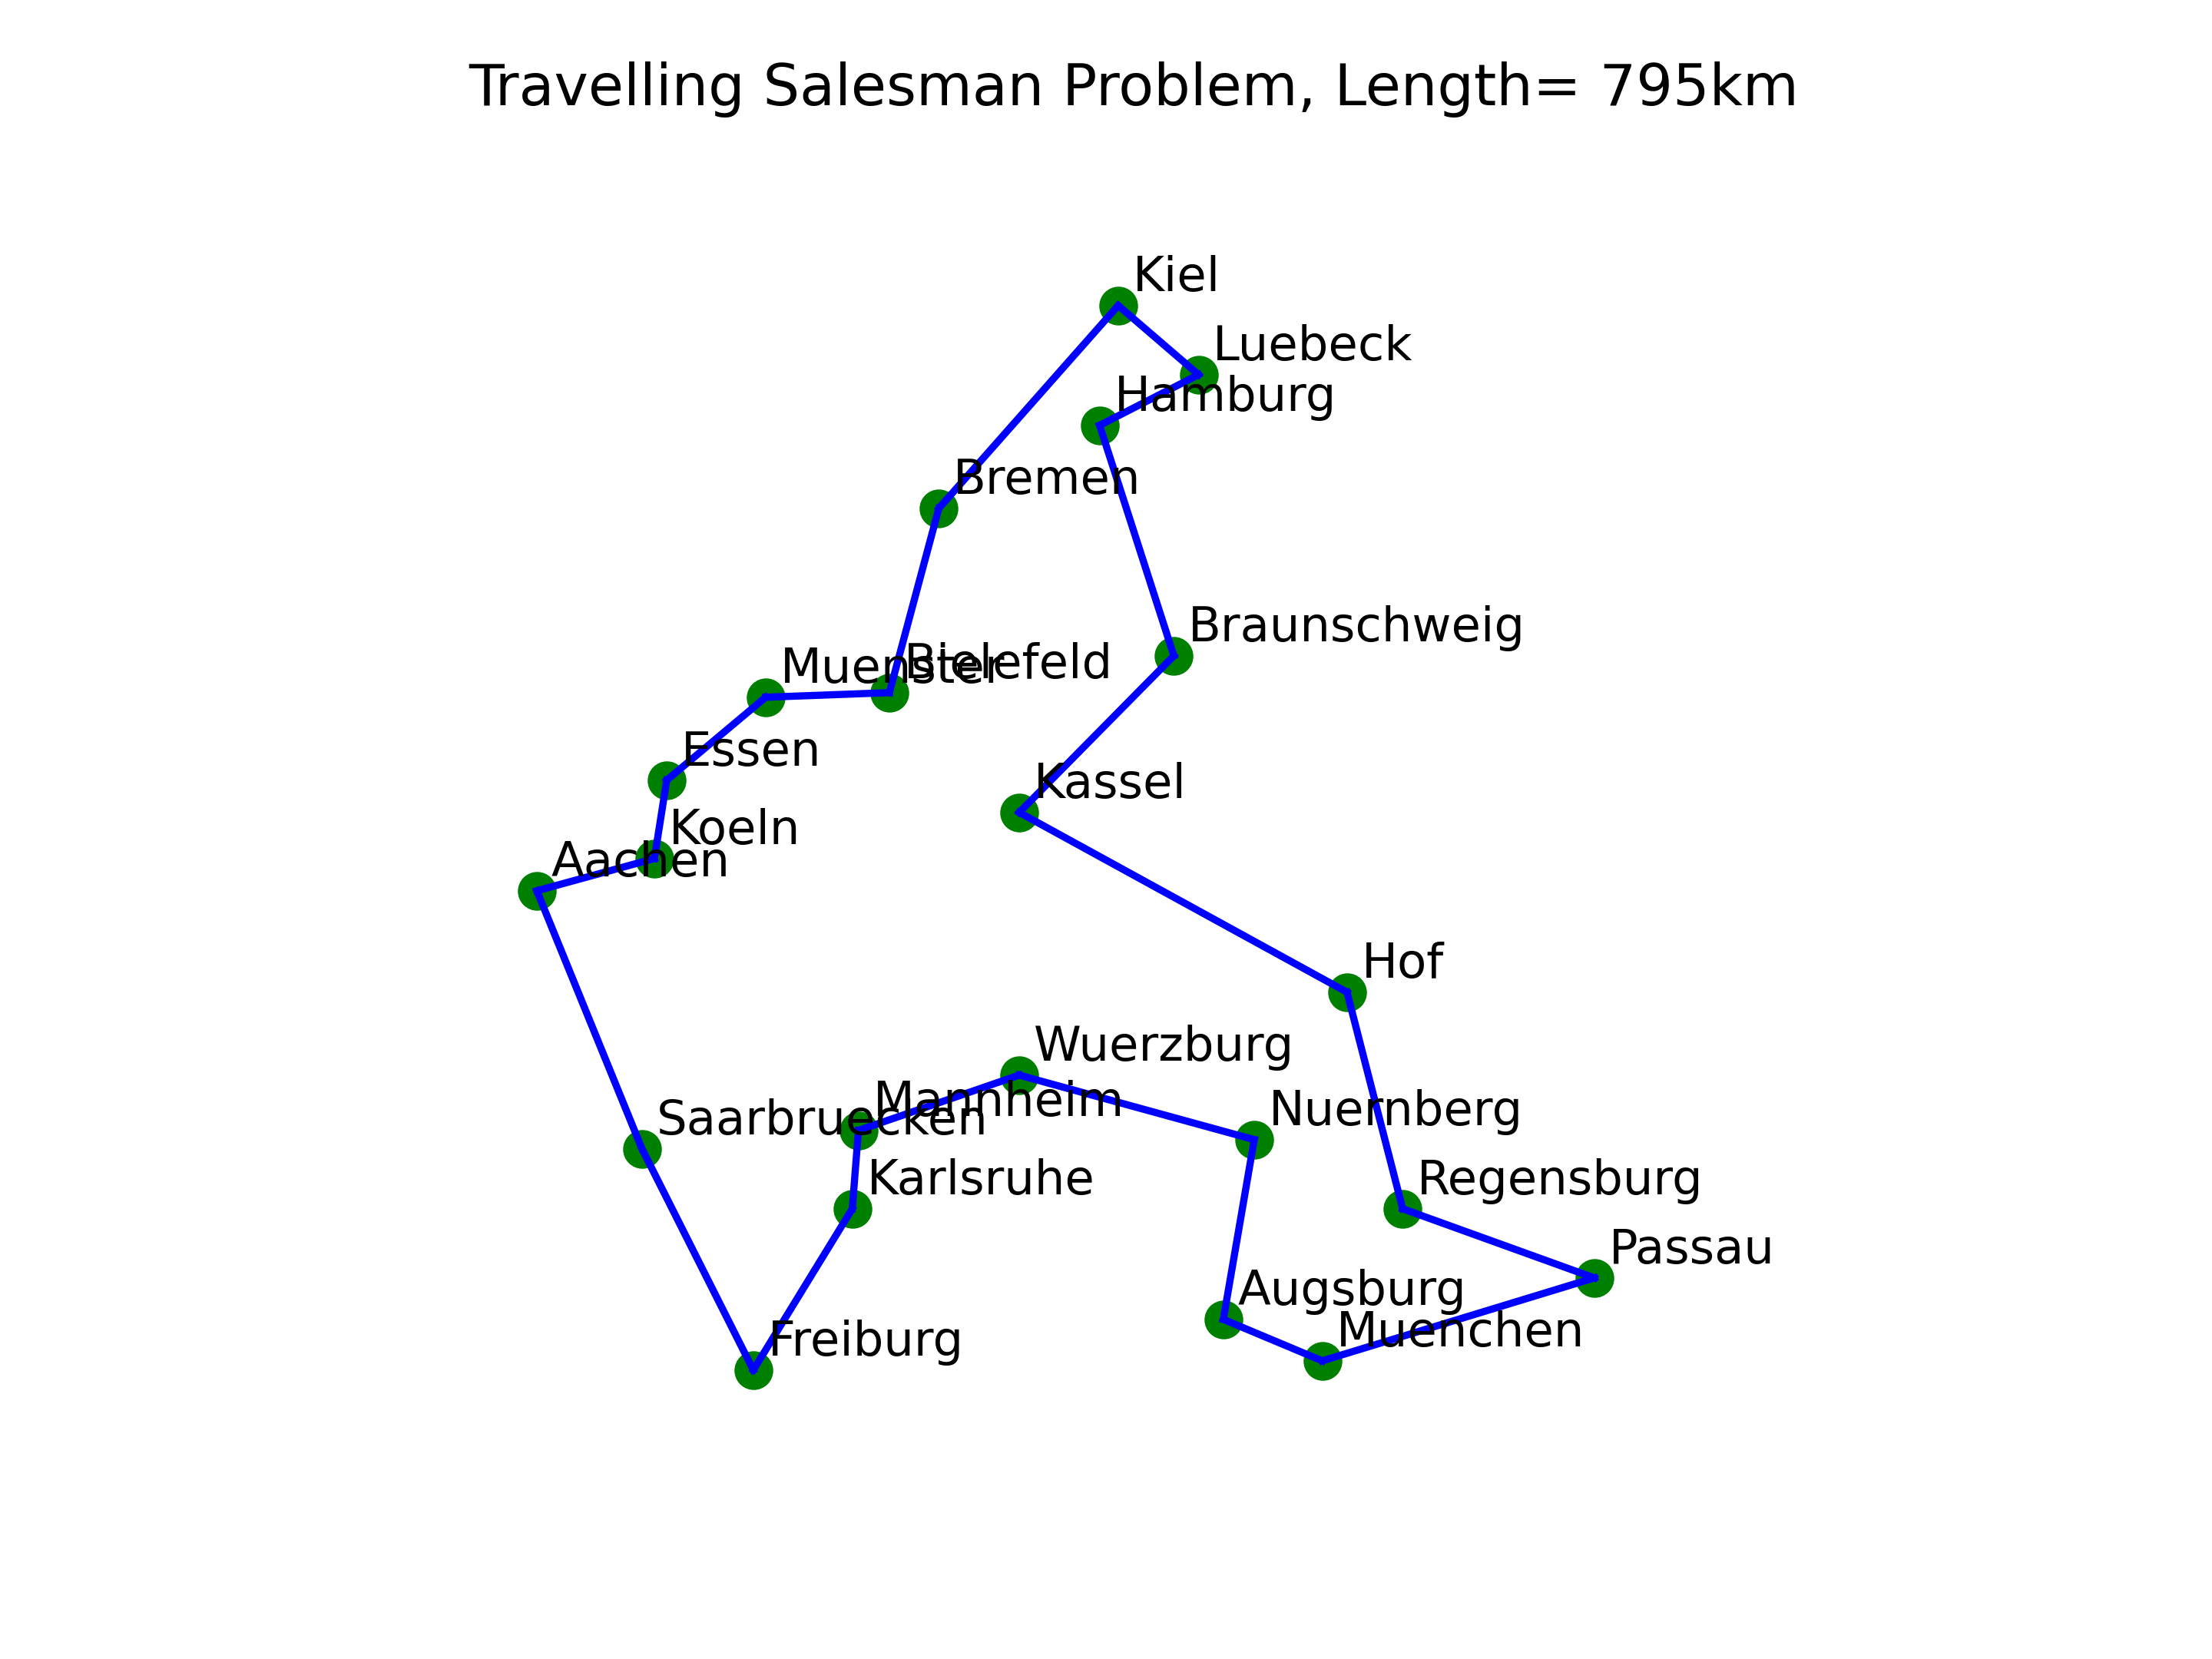
\includegraphics[width=0.80\textwidth]{../results/tsp_1.png}
    \captionof{figure}{Optimized route after 50000 iterations}
    \label{fig:tsp_1}
\end{center}
